\section*{Difracción de Fraunhofer}

\item
\begin{enumerate}
	\item Considere la figura de difracción de Fraunhofer producida por una rendija de ancho $b$ ubicada entre dos lentes convergentes y centrada en el eje óptico del sistema.
La fuente puntual de longitud de onda $\lambda$ se coloca en el foco de la primera lente. 
	\begin{enumerate}
		\item ¿Dónde se coloca la pantalla de observación?
		\item Calcule la posición de los máximos y de los mínimos de irradiancia, el ancho angular de la campana principal de difracción y de los máximos secundarios. 
		\item Calcule la relación de irradianciaes entre el máximo principal y el primer máximo secundario. 
		\item Grafique la irradiancia sobre la pantalla.
		¿En función de qué variables lo hace?
		¿Podría haber elegido otras?, ¿cuáles?
		\item Discuta cómo se modifican los parámetros de la figura de difracción si se cambia: 1) el ancho de la ranura, 2) la longitud de onda, 3) si se coloca una fuente policromática. 
	\end{enumerate}
	\item Idem a), si la fuente se encuentra en el plano focal de la primera lente, a una altura $h$ del eje óptico. 
	\item Idem b), si la ranura se centra a una altura $h'$ del eje óptico. 
\end{enumerate}



\item Una rendija de \SI{50}{\micro\metre} de ancho se encuentra entre dos lentes delgadas convergentes de igual distancia focal, y está iluminada por ondas planas, de longitud de onda $\lambda = \SI{5000}{\angstrom}$.
La distancia entre el primer mínimo a la izquierda del máximo principal y el tercer mínimo a su derecha es de \SI{3}{\milli\metre}.
Además, el primer mínimo a la izquierda está ubicado \SI{3}{\milli\metre} a la derecha del eje óptico.
\begin{enumerate}
	\item ¿Cuál es la distancia focal de las lentes? 
	\item ¿Dónde se encuentra la fuente?
	¿Dónde el máximo principal? 
\end{enumerate}



\item
\begin{enumerate}
	\item (*) Hallar el patrón de irradianciaes de una abertura rectangular de lados $a$ y $b$, que se encuentra a distancia $D$ de una pantalla.
	Considere incidencia normal. 
	\item (*) Idem para una abertura circular de radio $a$.
\end{enumerate}



\item (*)
\begin{minipage}[t][1.2cm]{0.65\textwidth}
Hallar el campo eléctrico, como función de las coordenadas sobre la pantalla, para las configuraciones de la figura, las que se encuentran a distancia $D$ de la pantalla.
La luz es monocromática de longitud de onda $\lambda$ e incide normalmente sobre las aberturas. 
\end{minipage}
\begin{minipage}[c][1.5cm][t]{0.3\textwidth}
	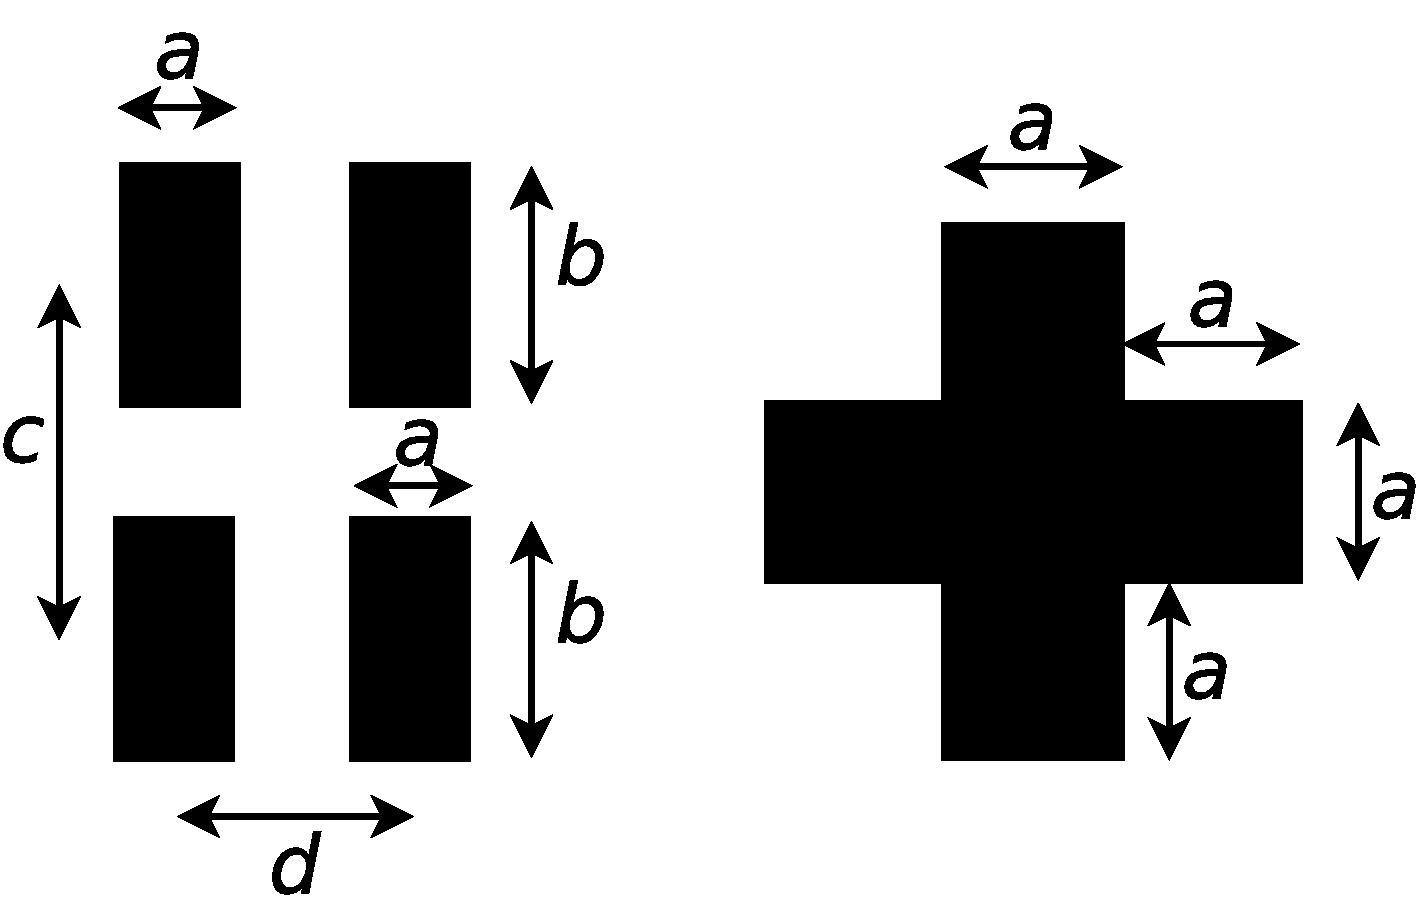
\includegraphics[width=\textwidth]{ej5-35}
\end{minipage}
